\documentclass[10pt, letterpaper]{paper}
\usepackage{graphicx}
\usepackage{amssymb}
\usepackage{amsmath}
\usepackage{listings}
 
\title{ Problem Set \#1 }
\author{ Timothy Schwieg }	
\date { July 13th 2017 }

\begin{document}

\maketitle

\section*{Question 1}
Relational Databases are far more effective than spreadsheets when multiple tables that may have dependencies are required. 
For example, in an attempt to fix their parking woes, the University of Central Florida may wish to track which people are parking in which lots and for what amounts of time.
To get at this data, they will record the identification numbers of the cars parked in various lots around campus. Three tables will be formed to store the information: Vehicles, Garages, and Students
\newline \newline
The table titled Vehicles contains VehID which is the primary key for the table; CarType, the type of car parked, StudentID, the NID of the student who purchased the decal, a key for the students table; GarageID, the ID of the Garage where the vehicle was parked; and Date, the timestamp of when the vehicle was recorded parked.
\newline 
The table titled Garages contains GarageID, the primary key; Location, describing where the garage is located; and MaxSize, the maximum number of parking spots in the garage.
\newline
The table titled Students contains studentID, the primary key for the student; Schedule, a simplified version of their schedule showing the class they were attending; Residency, denoting if they live on campus or off. 

\begin{figure}[h!]
\centering
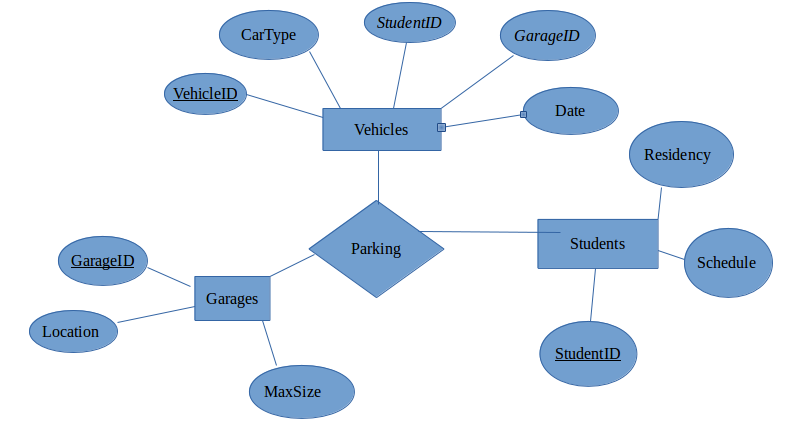
\includegraphics[width=0.8\textwidth]{ERDiagram.png}
\caption{ ER Diagram }
\end{figure}


Dependencies are avoided by placing the data into three separate tables. If a student were to drive multiple cars to campus, all will only refer to one element in Students. Likewise, changes to the garages need only to be made in one place, and they will be altered in all parking records.


\subsection*{Code}
\lstinputlisting[language=SQL]{CreateParkingDataBase.sql}

This yeilds the following output:
\newline

\lstinputlisting{output.txt}


\section*{Question 2}

If we consider the set corresponding to TableOne as A, and the set for TableTwo to be B. The elements of both sets are tuples that areindexed by the natural numbers, such that if $a \in A$, then $a[1]$ would describe the t1\_id field for the element a.
\newline

SELECT * FROM tableone JOIN tabletwo; is equivalent to A x B
\newline


SELECT * FROM tableone JOIN tabletwo WHERE tableone.t1\_id = tabletwo.t2\_id is equivalent to $\{ (a,b) | a \in A, b \in B, a[1] = b[1]\}$
 \newline
 
SELECT * FROM tableone JOIN tabletwo WHERE tableone.t1\_subid = tabletwo.t2\_subid is equivalent to $\{ (a,b) | a \in A, b \in B, a[2] = b[2]\}$
 \newline
 
SELECT * FROM tableone JOIN tabletwo WHERE tableone.t1\_var1 = tabletwo.t2\_var1 is equivalent to $\{ (a,b) | a \in A, b \in B, a[3] = b[3]\}$
 


\section*{Question 3}
\subsection*{a.}
\begin{figure}[h!]
\centering
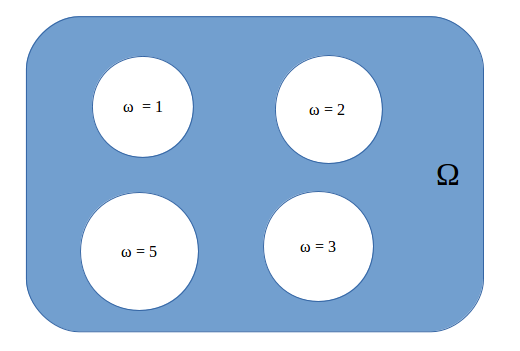
\includegraphics[width=0.8\textwidth]{VennDiagram.png}
\caption{ Venn Diagram of Primary Events }
\end{figure}

Since there is only one dice toss in our universe, it only allows for four possible outcomes: 
$$\Omega = \{1,2,3,5\}$$ In this universe, the simple events are disjoint because the die can only land on one of the possible sides. Thus the probability of rolling an intersection between these simple events is zero. This implies that the probability of rolling a union between the events is just the sum of the probability of those events.

$$P( \omega = 1 \cup \omega = 3 ) = P( \omega = 1 ) + P( \omega = 3 )$$

\subsection*{b.}
$$X:\Omega \rightarrow {\rm I\!R} = 
\begin{cases} 
      1 & \omega = 1 \\
      2 & \omega = 2 \\
      3 & \omega = 3 \\
      5 & \omega = 5
   \end{cases}$$

\subsection*{c.}
$$p_X (x) = \frac{1}{4} \text{ for x = } 1,2,3,5 ; p_X (x) = 0 \text{ otherwise}$$

$$F_X(x) = \sum_{i = 1}^{x} p_X (i) = \begin{cases} 
		0 		  & x < 1\\
      \frac{1}{4} & x = 1 \\
      \frac{1}{2} & x = 2 \\
      \frac{3}{4} & x = 3 \\
      1 & x > 3
   \end{cases}$$
   
\begin{figure}[h!]
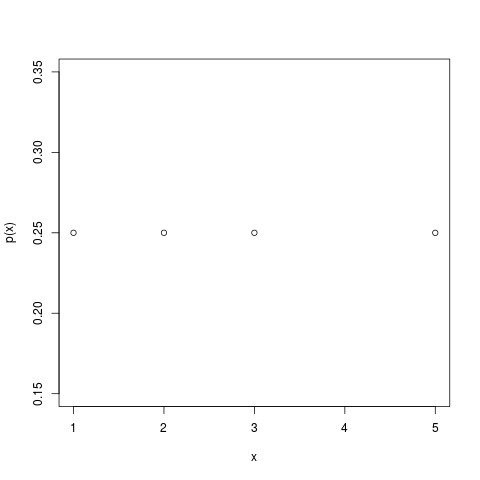
\includegraphics[width=0.8\textwidth]{pmfPlots.png}
\caption{ $p_X (x)$ }
\end{figure}

\begin{figure}[h!]
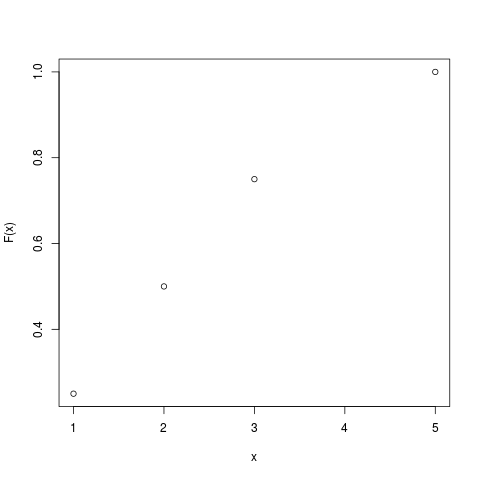
\includegraphics[width=0.8\textwidth]{CumDistPlot.png}
\caption{ $F_X (x)$ }
\end{figure}
   
$$E[X] = \sum_{ x \in \mathbb{N}}^{} x p_X (x) = \frac{1}{4} + \frac{1}{2} + \frac{3}{4} + \frac{5}{4} = \frac{11}{4}$$

$$Var(X) = E[X^2] - E[X]^2 = \sum_{ x \in \mathbb{N}}^{} x^2 p_X (x) - \frac{121}{16} = \frac{1}{4} + 1 + \frac{9}{4} + \frac{25}{4} - \frac{121}{16} = \frac{35}{16}$$

\subsection*{d.}
\begin{table}[h!]
\centering
\begin{tabular}{|l|r|r|r|r|r|r|r|r|r|r|}
\hline
S & $<$ 2 & 2 & 3 & 4 & 5 & 6 & 7 & 8 & 10 & $>$ 10 \\
\hline
$p_S (s)$ & 0 &  $\frac{1}{16}$ & $\frac{1}{8}$ & $\frac{3}{16}$ & $\frac{1}{8}$ & $\frac{3}{16}$ & $\frac{1}{8}$ & $\frac{1}{8}$ & $\frac{1}{16}$ & 0\\
\hline

\end{tabular}
\end{table}

\begin{figure}[h!]
\centering
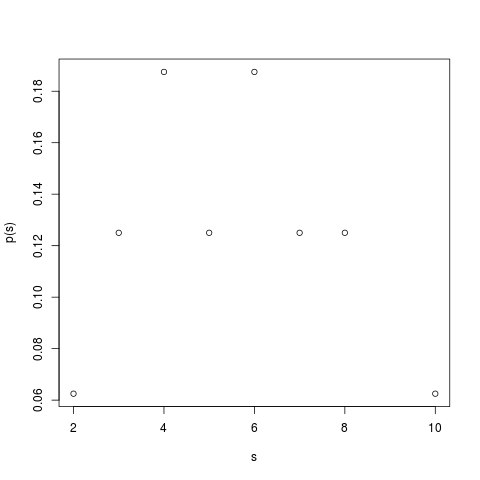
\includegraphics[width=0.8\textwidth]{Sumplot.png}
\caption{ $p_S (s)$ }
\end{figure}


$$E[S]= \sum_{ s \in \mathbb{N}}^{} s p_S (s) = \frac{1}{16} + \frac{1}{4} + \frac{9}{16} + \frac{5}{8} + \frac{9}{8} + \frac{7}{8} + 1 + \frac{5}{8} = \frac{41}{8}$$

$$V(S) = \sum_{ s \in \mathbb{N}}^{} s^2 p_S (s) - \frac{1681}{64} = \frac{1}{4} + \frac{9}{8} + 3 + \frac{25}{8} + \frac{27}{4} + \frac{49}{8} + 8 + \frac{25}{4} - \frac{1681}{64} = \frac{535}{64}$$

We were able to easily create the closed form for the probability mass function because we assumed independence between the rolls of the dice, if rolling the dice gave us information about the probabilities of the die, it would not be independent, and the mass function for the mass would not be so simple to calculate.

\subsection*{e.}
The odds are given by $\frac{P(S=s)}{P( S \neq s )}$ So the odds for $S = 6$ are given by: $\frac{P(S=6)}{P( S \neq 6 )} = \frac{3}{13}$

\subsection*{f.}

For the event to be considered fair, the expected value must equal zero. So for some payoff x, the equation: $ x P(S = 6 ) - 1 P( S \neq 6 ) = 0 $ so $x = \frac{P( S \neq 6)}{P( S = 6 ) }$ and thus: $x = \frac{ 13}{3}$

\end{document}
